We aimed to determine and understand the influence of risk group turnover on
the contribution of the highest risk group to the overall epidemic,
as measured by the transmission population attributable fraction (TPAF).
However, to understand the underlying mechanism,
we first examined the influence of turnover on
the equilibrium incidence and prevalence projected among risk groups, as well as overall.
% SB: Is this STI incidence and prevalence? I would keep specifying so all are clear here.
Since the influence may depend on the duration of infectiousness,
we also explored the sensitivity of these results to different treatment rates.
Next, we examined how turnover may influence
inferred model parameters through model fitting.
Finally, we compared the TPAF of the highest risk group with and without turnover,
before and after model fitting.
Our experiments can be summarized as in Table~\ref{tab:exp}.
% LW: This paragraph is essentially ur objective statement,
%     which can be merged with the last paragraph of the Intro.
\begin{table}
  \centering
  \caption{Summary of experiments}
  \label{tab:exp}
  \small
\begin{tabular}{clllll}
 	\toprule
 	Experiment & Outputs               & Stratifications   & Turnover    & Treatment      & Fitting             \\
 	\midrule
	   1.1.    & prevalence            & overall           & any vs none & fixed, 2 rates & none                \\
	   1.2.    & prevalence, incidence & overall, by group & varied      & fixed, 1 rate  & none                \\
	   1.3.    & prevalence, incidence & overall, by group & varied      & varied         & none                \\
 	\midrule
	   2.      & inferred contact rate & by group          & any vs none & fixed, 1 rate  & prevalence by group \\
 	\midrule
	   3.1.    & TPAF                  & highest risk      & any vs none & fixed, 1 rate  & none                \\
	   3.2.    & TPAF                  & highest risk      & any vs none & fixed, 1 rate  & prevalence by group \\
 	\bottomrule
\end{tabular}\\[1em]
\footnotesize{TPAF: transmission population attributable fraction}

\end{table}
% ==================================================================================================
\subsection{Model \& Simulations}\label{ss:model-sim}
To run our experiments,
we developed a deterministic single-sex SIT model
% SB: I think first time need to say susceptible, infected,
%     treated given we are also talking about STI here.
which simulates transmission in a population with heterogeneity in risk.
The model is not representative of a specific infection
% SS: I think it might be easier to follow if it did.
%     I think it could be used as an example to thread across
%     and then in the discussion go into how this would be similar/different for another infection
%     (which parameters would likely change,
%     whether we would anticipate that the impact of turnover would be similar, different)
% SB: I get saying any STI—but some are curative and some aren’t. ie, you can treat some
%     folks but the infection may be sustained and in others it is totally gone.
%     So just ask the question as whether we want to specify more about which type of STI
%     might be included in a model like this.
but includes balancing contacts
as per sexually transmitted infections \citep{Garnett1994}.
% SB: Not sure what this means.
The model includes three health states:
susceptible~$\mathcal{S}$, infectious~$\mathcal{I}$, and treated~$\mathcal{T}$
(Figure~\ref{fig:health-states}),
and $G = 3$ levels of risk:
high~$H$, medium~$M$, and low~$L$.
Risk strata are defined by different number of contacts per year
so that individuals in risk group $i$ are assumed to
form contacts at a rate $C_{i}$ per year.
The probability of contact formation $\rho_{ik}$ between individuals in group $i$
and individuals in risk group $k$ is assumed to be
proportionate to the total number of available contacts within each group:
\begin{equation}
  \rho_{ik} = \frac
    {C_k x_k}
    {\sum_{\mathrm{k}}C_{\mathrm{k}} x_{\mathrm{k}}}
    \label{eq:rho}
\end{equation}
\begin{figure}
  \centering
  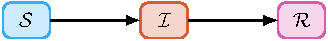
\includegraphics[width=0.4\linewidth]{health-states}
  \caption{Modelled health states.
  $\mathcal{S}$: susceptible;
  $\mathcal{I}$: infected;
  $\mathcal{T}$: treated;
  $\lambda$: force of infection;
  $\tau$: treatment.}
  \label{fig:health-states}
\end{figure}
\par
The biological probability of transmission is defined as $\beta$ per contact.
Individuals transition from the
infectious $\mathcal{I}$ to susceptible $\mathcal{S}$ health-state
% SS: Check: Not from the susceptible to the infectious?
via a force of infection $\lambda$ per year, per susceptible in risk group $i$:
\begin{equation}
  \lambda_{i} =
  C_{i} \sum_k \rho_{ik} \thinspace  \beta \thinspace \frac{\mathcal{I}_k}{x_k}
  \label{eq:foi}
\end{equation}
Individuals are assumed to transition from the
infectious $\mathcal{I}$ to treated $\mathcal{T}$ health-state
at a rate $\tau$ per year, reflecting diagnosis and treatment.
The treatment rate is not stratified by risk group.
Individuals in the treated $\mathcal{T}$ health-state are not infectious nor susceptible,
and individuals cannot become re-infected.
% SS: What seems confusing to me at this point is that
%     given the lack of specificity of the infection of interest,
%     the R assumptions seem potentially overly simplistic
%     given that with most STIs there is unlikely to be immunity following recovery
%     and in the case of HIV, treatment (if considered R) may be stopped/incomplete
%     and then they may not be susceptible, but certainly transmittable.
\par
% LW: For this paragraph and the next, have a sub-heading such as:
%     "implement turn-over in in SIT model."
As described in Section~\ref{s:system}, individuals
enter the model at a rate $\nu$,
exit the model at a rate $\mu$,
and transition from risk group $i$ to group $j$ at a rate $\phi_{ij}$.
The turnover rates $\phi$ and
distribution of individuals entering the model by risk group $\bm{\hat{e}}$
were computed using the methods outlined in
Section \ref{sss:params-turnover}
and the following assumptions.
% SB: Do we need to explain why we made these assumptions? Or provide refs?
First, we assumed that
the proportion of individuals entering each risk group $\bm{\hat{e}}$
was equal to the proportion of individuals across risk groups in the model $\bm{\hat{x}}$.
% LW: And another strong assumption which was implicit here is that u assume
%     the rate of turn over to be the same irrespective of disease status.
%     And I think it is critical to make it explicit.
%     So S, I, T all have the same turn over rate,
Second, we assumed that
the average duration spent in each risk group $\bm{\delta}$ is known.
Third, we assumed that
the absolute number of individuals moving between two risk groups in either direction is balanced.
% LW: I would think this is a very strong assumption.
%     It is essentially saying the turn-over system consistently
%     *swap* individuals in two risk groups.
% HM: Not fully understand how does this assumption work?
%     If high risk group has 10 individuals move to medium group,
%     medium group will move 10 individuals to high risk? This is independent from population entry?
The system of equations which results from these assumptions
is given in Appendix~\ref{aa:eqs-turnover}.
To meet all three conditions, there is only one possible value
for each element in $\phi$ and $\bm{\hat{e}}$
-- i.e.\ $A$ is full rank.
In other words, by specifying these three conditions,
we ensure that a unique set of $\phi$ and $\bm{\hat{e}}$ is computed.
\par
Using the above three assumptions,
we need to specify the values of $\bm{\hat{x}}$, $\bm{\delta}$, $\nu$, and $\mu$.
Such parameters could be derived from data as described in Section \ref{sss:params-turnover};
however, in this experiment, we use the illustrative values summarized in
Table~\ref{tab:params}.
% LW: After read the whole results section,
%     I think experiment 2 and 3.2 followed values specified in Table 3.
%     But experiment 1 and 3.1 explored a wide range of
%     turn-over and treatment rates.
%     it is unclear what do u refer to when u said “this experiment”.
%     Given the organization and length – by the time I reached results of Experiemnt 2,
%     I almost forgot under which values they were done – as the section preceed it
%     explored a range of values of turn-over rate and treatment rate.
After resolving the system of equations,
$\bm{\hat{e}}$ is equal to $\bm{\hat{x}}$ (assumed), and $\phi$ is:
\begin{equation} % TODO: automate this output
\label{eq:phi-values}
\phi = \left[\begin{array}{ccc}
*      & 0.0833 & 0.0867 \\
0.0208 & *      & 0.0158 \\
0.0058 & 0.0042 & *      \\
\end{array}\right]
\end{equation}
\begin{table}
  \centering
  \caption{Model parameters.
    All rates have units $\mathrm{year}^{-1}$; durations are in $\mathrm{years}$;
    parameters stratified by risk group are written [high, medium, low] risk.}
  \label{tab:params}
  \begin{tabular}{clc}
	\toprule
	    Symbol     & Description                                                     &            Value             \\
	\midrule
	 $\bm{\beta}$  & transmission probability per contact                            &            $0.03$            \\
	    $\tau$     & rate of treatment initiation among infected                     &            $0.1$             \\
	    $N_0$      & initial population size                                         &            $1000$            \\
	\midrule
	$\bm{\hat{x}}$ & proportion of system individuals by risk group                  & $[ 0.05 \es 0.20 \es 0.75 ]$ \\
	$\bm{\hat{e}}$ & proportion of entering individuals risk by risk group           & $[ 0.05 \es 0.20 \es 0.75 ]$ \\
	$\bm{\delta}$  & average duration spent in each risk group                       &    $[ 5 \es 15 \es 25 ]$     \\
	     $C$       & rate of contact formation among individuals in each risk group  &     $[ 25 \es 5 \es 1 ]$     \\
	    $\nu$      & rate of population entry                                        &            $0.05$            \\
	    $\mu$      & rate of population exit                                         &            $0.03$            \\
	\bottomrule
\end{tabular}
  %% SS: All of this seems a little hard to follow in terms of the infection,
  %% b/c it seems to indicate that there is an underlying infection of interest,
  %% but it is not being stated.
\end{table}
\par
We then simulated epidemics using these parameters.
The model was initialized with $N_0 = 1000$ individuals
who are distributed across risk groups according to $\bm{\hat{x}}$.
We seeded the epidemic with
one infectious individual in each risk group at $t = 0$.
There were no treated individuals at the start of the epidemic,
and so all individuals except the 3 infectious individuals were susceptible.
We numerically solved the system of ordinary differential equations
in Python%
\footnote{Code for all aspects of the project is available at:
  \href{https://github.com/c-uhs/turnover}{\texttt{https://github.com/c-uhs/turnover}}}
using Euler's method with a time step of $dt = 0.1$ years.
The full system of model equations is given in Appendix~\ref{aa:eqs-model}.
All comparative analyses are then conducted at equilibrium,
defined as a steady state with $<$1\% difference in incidence per year.
% ==================================================================================================
\subsection{Experiment 1: Influence of turnover on equilibrium incidence and prevalence}
\label{ss:exp-1}
Experiment 1 examined the influence of turnover on
equilibrium incidence and prevalence, where
incidence is defined as $\lambda_i$ from Eq.~(\ref{eq:foi}), and
prevalence is defined as $\hat{\mathcal{I}}_i = \dfrac{\mathcal{I}_i}{\mathcal{X}_i}$.
% --------------------------------------------------------------------------------------------------
\paragraph{Experiment 1.1: Overall prevalence with vs without turnover}
\label{p:exp-turnover-simple}
First, we compare the overall prevalence predicted by the model with and without turnover.
The model with turnover is as described above.
The model without turnover has all rates $\phi = 0$.
Following Eq.~(\ref{eq:duration-group}),
this means that in the model without turnover,
the time spent within each risk group is equal to
the average duration in the modelled population $\mu^{-1}$.
The comparison of prevalence is repeated for two different treatment rates,
in order to illustrate variability in the relative difference.
% --------------------------------------------------------------------------------------------------
\paragraph{Experiment 1.2: Influence of turnover rates on incidence and prevalence}
\label{p:exp-turnover-1D}
%% SM: start by something like this to orient the reader and help with interpretation before results section
%% JK: I agree this could be useful, but then we go back-and forth between
%% implementation ("controlled by a single parameter") and
%% an overview of the experiment ("influence of turnover on ...")
%% I'd rather introduce how turnover is controlled via duration in high risk group
%% after noting why we cannot simply scale the rates proportionally with a single parameter.
Second, we determined the influence of different turnover rates on
equilibrium incidence and prevalence
at a fixed duration of infectiousness (treatment rate).
As in similar experiments \citep{Zhang2012,Henry2015},
the rates of turnover were scaled by a single parameter.
However, because the model used here has $G = 3$ risk groups,
multiplying by a set of base rates $\phi$ by a scalar factor
would have resulted in changes to the relative population size of risk groups $\bm{\hat{x}}$.
Thus, we controlled the rates of turnover using
the duration of individuals in the high risk group $\delta_H$,
such that a shorter period of time in the high risk group
corresponded to higher rates of turnover among all groups.
The duration of individuals in the medium risk group $\delta_M$
was then defined as a value between $\delta_H$ and the maximum duration $\mu^{-1}$
which scales with $\delta_H$ following the equation:
$\delta_M = \delta_H + \kappa \left(\mu^{-1} - \delta_H\right)$, with $\kappa = 0.3$.
The duration of individuals in the low risk group $\delta_L$
similarly scaled with $\delta_H$,
but the value was not required to calculate $\phi$;
it can be determined from $\phi$ afterwards
using Eq.~(\ref{eq:duration-group}).
In this way, each value of $\delta_H$ was used to define a unique set of turnover rates $\phi$
whose elements all scaled inversely with the duration in the high risk group $\delta_H$.
The value of $\delta_H$ was then varied from 33~to~3 years
to examine the influence of different turnover rates.
% --------------------------------------------------------------------------------------------------
\paragraph{Experiment 1.3: Influence of turnover rates at various treatment rates}
\label{p:exp-turnover-2D}
Next, we conducted a 2-way sensitivity analysis to examine how
the influence of turnover might vary at different treatment rates.
The treatment rate controls the duration of infectiousness $\delta_{\mathcal{I}}$
as in $\delta_{\mathcal{I}} = \tau^{-1}$.
Treatment rate $\tau$ was varied from 1~to~0.05,
implying a duration of infectiousness of 1~to~20 years.
The duration of time spent in the high risk group $\delta_H$
was varied from 33~to~3 years as in Experiment 1.2.
We examined the influence of the rates of turnover on
equilibrium prevalence and incidence across the
range of treatment rates using multiple 1D plots and 2D surface plots.
% ==================================================================================================
\subsection{Experiment 2: Inferred risk heterogeneity with vs without turnover}
\label{ss:exp-infer}
In Experiment 2, we examined the influence of turnover on
the parameter values inferred via model fitting.
Specifically, we fit the model to
20\% infection prevalence among the high risk group,
3\% among the low risk group,
and 5\% overall,
with and without turnover .
We fit the contact rates $C$ of all risk groups
by minimizing the negative log-likelihood of each predicted prevalence versus the target.%
\footnote{Sample sizes of 50, 750, and 1000 were assumed to generate binomial distributions
  for the high, low, and overall prevalence targets respectively,
  and the minimization was performed using
  the SLSQP method~\citep{Kraft1988} from the SciPy Python package
  (\href{https://docs.scipy.org/doc/scipy/reference/generated/scipy.optimize.minimize.html}
        {\texttt{scipy.optimize.minimize}}).}
We then compared the inferred contact rates $C$
in the model with versus without turnover.
The ratio of fitted (or posterior) contact rates $C_H~/~C_L$
represents the degree of risk heterogeneity in the population,
after fixing all other parameters,
which produces the given infection prevalence.
% ==================================================================================================
\subsection{Experiment 3: Influence of turnover on the TPAF of the high risk group}
\label{ss:exp-tpaf}
Finally, Experiment 3 sought to examine how
the estimated contribution of highest risk group to overall transmission,
as measured by the transmission population attributable fraction (TPAF),
varies with versus without turnover.
The TPAF of a risk group $i$ is defined as:
\begin{equation}
  \textsc{tpaf}_i(t) = \frac{I_0(t) - I_i(t)}{I_0(t)}
\end{equation}
where $I_0(t)$ is the cumulative number of new infections
by time $t$ under usual conditions,
and $I_i(t)$ is the cumulative number of new infections
assuming no transmission from risk group $i$.
Both $I_0(t)$ and $I_i(t)$ are calculated
starting from a system at equilibrium.
There are two ways to consider the comparison of TPAF with versus without turnover;
these are illustrated in Figure~\ref{fig:exp-tpaf},
and explained in the following sections.
\begin{figure}
  \centering
  \begin{subfigure}{0.48\linewidth}
    \centering
    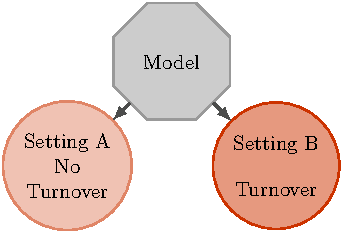
\includegraphics[width=0.7\linewidth]{tpaf-raw}
    \caption{Experiment 3.1: same parameters, different prevalence (no model fitting)}
  \end{subfigure}
  \begin{subfigure}{0.48\linewidth}
    \centering
    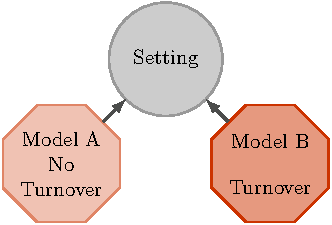
\includegraphics[width=0.7\linewidth]{tpaf-fit}
    \caption{Experiment 3.2: same prevalence, different parameters (fitted model)}
  \end{subfigure}
  \caption{Two approaches to comparing TPAF with and without turnover}
  \label{fig:exp-tpaf}
\end{figure}
% --------------------------------------------------------------------------------------------------
\paragraph{Experiment 3.1: Two settings}
\label{p:exp-tpaf-raw}
First, we compared two hypothetical settings,
which had identical populations (including behaviour), except that
setting A had no turnover: $\phi = 0$, while
setting B had turnover: $\phi$ from Eq.~(\ref{eq:phi-values}).
As a result, model parameters were identical (except turnover),
but the infection prevalence predicted for each setting was different.
Following equilibration of the model in both settings,
the TPAF of the high risk group was then estimated.
% --------------------------------------------------------------------------------------------------
\paragraph{Experiment 3.2: Two models}
\label{p:exp-tpaf-fit}
Second, we compared two models,
which were identical in structure except that
Model A had no turnover and Model B had turnover.
In this case, both models were fitted to
the same ``setting'', as defined by overall and group-specific equilibrium infection prevalence
(from Experiment~2).
As a result, prevalence was the same in both models,
but the group-specific contact rates inferred via fitting were different.
As before, the TPAF of the high risk group was then estimated
in each model after equilibration.
